\section{calculation}
In this simplified situation, there is no wall and only one other pedestrian $\beta$ at position $(-\frac{\sqrt{2}}{5}, \frac{\sqrt{2}}{5})$ which exert expelling force to $\alpha$.  The exit is reduced to one point $E(4,4)$.  Their positions at $t=0$ is shown in the drawing below:\\

\begin{figure}
\centering
{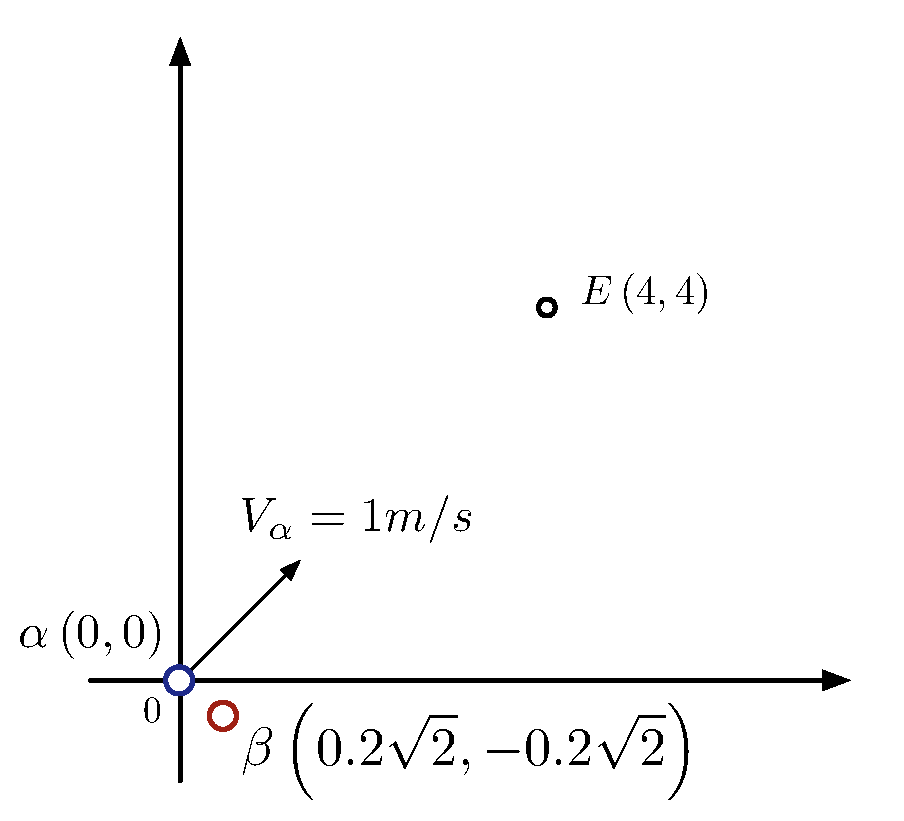
\includegraphics[scale=0.45]{calculation.pdf}} 
\caption{\small{}\label{calc}}
\end{figure}

In addition, to complete the initial conditions, we need to know $\alpha$'s actual velocity at $t=0$, suppose $\overrightarrow{v_{\alpha}(0)}=(\frac{\sqrt{2}}{2}, \frac{\sqrt{2}}{2})$, also the average speed into the desired direction of motion $\overline{v_{\alpha}(0)}=0$.\\

With those numbers we can calculate the impatience factor 
 \begin{equation}
 n_{\alpha}(0)=1-\frac{\overline{v_{\alpha}(0)}}{v^{0}_{\alpha}(0)}=1-\dfrac{0}{v^{0}_{\alpha}(0)}=1
 \end{equation}

so 
 \begin{equation}
 v^{0}_{\alpha}(0)=[1-n_{\alpha}(0)]v^{0}_{\alpha}(0) + n_{\alpha}(0)v_{\alpha}^{max} = v_{\alpha}^{max}
 \end{equation}
 
Suppose $v_{\alpha}^{max}=3$, then 

 \begin{equation}
 	\vec{f^{0}_{\alpha}} \left( \vec{v_{\alpha}} \right) 
= 	\frac{1}{\tau_{\alpha}} \left( v^{0}_{\alpha} 
	\vec{e_{\alpha}} - \vec{v_{\alpha}} \right)
 \end{equation}
 
where $\tau_{\alpha}=1$,
 \begin{equation}
 \overrightarrow{f^{0}_{\alpha}}\overrightarrow{v_{\alpha}} = (\sqrt{2}, \sqrt{2})
 \end{equation}

Another part of $\alpha$'s acceleration is from the repelling force from $\beta$, in order to speed  up the calculation here we omit the not so important part in calculating $\overrightarrow{f_{\alpha \beta}}$.
Therefore,
 \begin{equation}
 \overrightarrow{f_{\alpha \beta}} = A^{2}_{\alpha} exp(\frac{r_{\alpha\beta}-d_{\alpha\beta}}{B^{2}_{\alpha}})\overrightarrow{n_{\alpha \beta}}
 \end{equation}
where $A^{2}_{\alpha}=3, B^{2}_{\alpha}=0.2, r_{\alpha\beta}=0.6, d_{\alpha\beta}=0.4$, and $\overrightarrow{n_{\alpha \beta}}=(-\frac{\sqrt{2}}{2}, \frac{\sqrt{2}}{2})$,
so 
 \begin{equation}
 \overrightarrow{f_{\alpha \beta}} = 8(-\frac{\sqrt{2}}{2}, \frac{\sqrt{2}}{2})
 \end{equation}
In all, the acceleration of $\alpha$ is 
 \begin{equation}
 \overrightarrow{f_{\alpha}(0)} = \overrightarrow{f^{0}_{\alpha}}\overrightarrow{v_{\alpha}} + \overrightarrow{f_{\alpha\beta}} = (-3\sqrt{2}, 5\sqrt{2})
 \end{equation}
Now we are ready to calculate where $\alpha$ is after $\bigtriangleup t=0.1$, if we assume $\alpha$ moves with a constant acceleration during that small time interval.
As the motion is in two dimensions, we need to calculate the displacement in $x$ and $y$ axis respectively.

 \begin{equation}
 r^{x}_{\alpha} = v^{x}_{\alpha} \bigtriangleup t + \frac{1}{2} f^{x}_{\alpha} \bigtriangleup t ^{2}
 \end{equation}
 
 For the y direction,
  \begin{equation}
 r^{y}_{\alpha} = v^{y}_{\alpha} \bigtriangleup t + \frac{1}{2} f^{y}_{\alpha} \bigtriangleup t ^{2}
 \end{equation}
 Therefore, $r_{\alpha}(0.1)= (0.05, 0.1)$